\documentclass{article}
\usepackage[utf8]{inputenc}
\usepackage[margin = 0.8in]{geometry}
\usepackage{graphicx}
\usepackage{amsmath, amssymb}
\usepackage{caption}
\usepackage{subcaption}
\usepackage{multirow}
\usepackage{multicol}
\usepackage{booktabs}
\usepackage{bm}
\setlength{\columnsep}{.75cm}
\usepackage{float}
\usepackage{graphicx}
\usepackage{stfloats}
\graphicspath{ {./images/} }
\setcounter{MaxMatrixCols}{15}

%\usepackage[parfill]{parskip}. %to not indent paragraph
\renewcommand\refname{References}
\restylefloat{table}


\title{LQR Control of a Nonlinear Quadrotor System}
\author{Keith Chester, Bob DeMont, Sean Hart}
\date{November 9th, 2021}

\begin{document}

\maketitle

\begin{figure}[h]
    \centering
    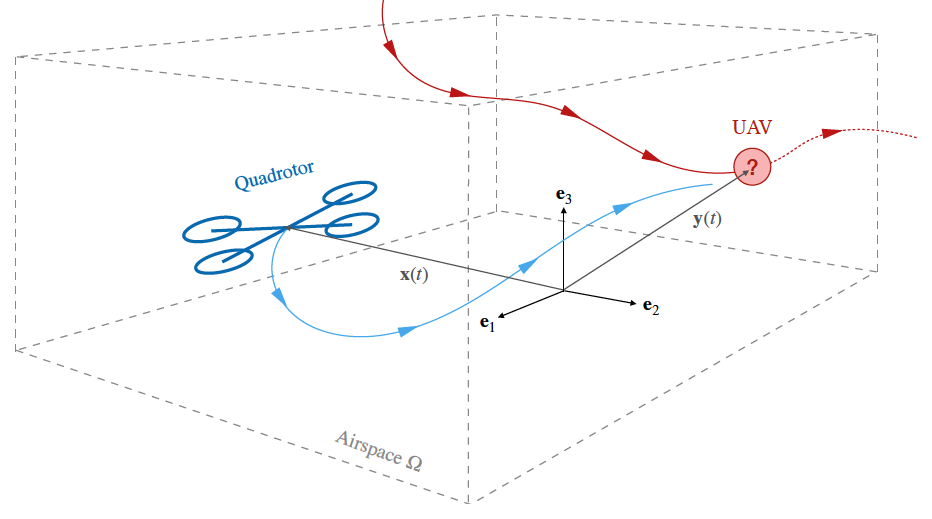
\includegraphics[width =0.75\textwidth]{images/ProjProbStmt.png}
    \label{fig:prob}
\end{figure}

\begin{multicols}{2}


\section*{Abstract}

The purpose of the project is to simulate the control and stable flight of an unmanned four rotor flying vehicle known as a quadrotor.  The problem is set into three goals: simulate and control the quadrotor hover in a stable configuration, chase an interloping quadrotor in flight and intercept, and return with the captured target quadrotor with randomized disturbance force while maintaining stable flight.

\section*{Situation/Problem}
The mission is defense of a designated airspace.  Our quadrotor is assigned to monitor a limited airspace, launch if an unidentified UAV enters that airspace, capture the target, and return to base.  If the target leaves the airspace before being captured, our quadrotor should return to base.  When captured, the target should be assumed to generate external forces on our UAV. The figure on the title page depicts the scenario.


\section*{Setup}

\noindent Coordinate frames are identified for the reference/inertial frame $E={e_1, e_2, e_3}$ at the center bottom of the airspace and the body frame $C={c_1, c_2, c_3}$.  All rotors are equidistant from the center of mass and in the same $c_1-c_2 $ plane as the body center of mass.  The external forces and moments on the system are represented by $\boldsymbol{r}$ and $\boldsymbol{n}$, where $\boldsymbol{r} = r_1 c_1 + r_2 c_2 + r_3 c_3$ and $\boldsymbol{n} = n_1 c_1 + n_2 c_2 + n_3 c_3$ directly applied to the center of mass. We are assuming that the torque of the rotor is proportionaly related to the input thrust via the constant $\sigma>0$, for $\tau_i = \sigma u_i$. We will be utilizing $\boldsymbol{I}$ as our diagonal inertial matrix where diagonal elements  $I_x, I_y $ and $I_z$ represent the mass moments of inertia about $c_1, c_2 $ and $c_3$ respectively.  For the purpose of our analysis we'll ignore the drag. The parameters for our state are described in table $\ref{table:Qparams}$.


\begin{table*}[t] %[bp]
\begin{centering}
\begin{tabular}{|cccc|}
\hline
Parameter & Value & Units  & Description  \\
\hline
 $l$  &  .02& m & Distance from center of mass to center of each rotor  \\
 $m$& .5 & kg &Total mass of quadrotor   \\
 $I_{x}$ & 1.24 kgm$^2 $ & s  & Mass moment of inertia about $c_1$ axis \\
 $I_{y}$ & 1.24 kgm$^2 $ & s  & Mass moment of inertia about $c_2$ axis \\
 $I_{z}$ & 1.24 kgm$^2 $ & s  & Mass moment of inertia about $c_3$ axis \\
$ g$ &9.81 & m/s$^2$ & Gravitational acceleration\\
$\sigma\ $& .01 & m & Proportionality constant relating $u_i $ to $\tau_i$\\
\hline
\end{tabular}
\caption{Quadrotor Parameters}
\label{table:Qparams}
\end{centering}
\end{table*}


\section*{General Approach}
We'll begin by generating the state space variables and defining the state space.  We'll prove controllability of the system and choose a controller methodology.  Using the controller, we will simulate hover as well as move to location and hover.  Finally we'll introduce external forces and moments that would be experienced simulating a target capture in the problem statement.  For ease of variable passing, our quadcopter will be represented as a structure in Matlab, with full state variables, A and B matrices, K gain matrix, $K_{capture}$ gain matrix (incorporating $n$ and $r$ forces and torques from the target) as well as characteristics for graphing (colors etc).

\section*{Methods}
We'll establish the state variable, $\mathbf{z}$ to represent the quadrotor's xyz center-of-mass position in the earth 
frame $\mathbf{x}=\begin{bmatrix}x_1 & x_2 & x_3\end{bmatrix}^T$; the roll, pitch, yaw angles in the earth frame, $\bm{\alpha}=\begin{bmatrix}\phi & \theta & \psi\end{bmatrix}^T$; the xyz linear velocities in the earth frame, $\mathbf{v}=\begin{bmatrix}v_1 & v_2 & v_3\end{bmatrix}^T$; and the angular accelerations $\bm{\omega}=\begin{bmatrix}\omega_1 & \omega_2 & \omega_3\end{bmatrix}^T$ in the earth roll pitch yaw directions. Our state variable then is $\mathbf{z}=\begin{bmatrix}\mathbf{x}&\bm{\alpha}&\mathbf{v}&\bm{\omega}\end{bmatrix}^T$. We define $\boldsymbol{\dot{z}}$ as $\begin{bmatrix} \mathbf{\dot{x}}&\bm{\dot{\alpha}}&\mathbf{\dot{v}}&\bm{\dot{\omega}} \end{bmatrix}^T$, with:

\begin{equation}
    \mathbf{\dot{x}} =\mathbf{v}
\end{equation}
\begin{equation}
    \bm{\dot{\alpha}} =\mathbf{T}^{-1}\bm{\omega}
\end{equation}
\begin{align}
    \mathbf{\dot{v}} =-ge_3+\frac{1}{m}\mathbf{R_{C/E}}(u_1+u_2+u_3+u_4)c_3 \nonumber\\ +\frac{1}{m}\mathbf{R_{C/E}}r
\end{align}
\begin{align}
    \bm{\dot{\omega}} =I^{-1}((u_2-u_4)lc_1+(u_3-u_1)lc_2 \nonumber\\ +(u_1-u_2+u_3-u_4)\sigma c_3+n-\omega \times I \omega)
\end{align}

\noindent ...where $\mathbf{R_{C/E}}$ is defined in the problem statement as the Euler rotation matrix from quadrotor frame $C$ to earth frame $E$ and $\mathbf{T}^{-1}$, also defined in the problem statement, relates the angular rate of change of the Euler angles based on the angular velocity of the quadrotor.

Our system is nonlinear because it is under-actuated; four actuators for six degrees of freedom. We can utilize linearization to simplify this model and approximate its behaviour for easier control. To do this, we wish to approximate our system as $\boldsymbol{\dot{z}}=\boldsymbol{A}\boldsymbol{x}+\boldsymbol{B}\boldsymbol{u}$. We derive the $\boldsymbol{A}$ matrix as the Jacobian of our $\boldsymbol{\dot{z}}$ by $\boldsymbol{z}$, and our $\boldsymbol{B}$ as the Jacobian of our $\boldsymbol{\dot{z}}$ by $\boldsymbol{u}$. Thus:

\begin{equation}
    \boldsymbol{A} = \begin{bmatrix}
        \frac{\partial \dot{x}}{\partial x} &
        \frac{\partial \dot{x}}{\partial y} &
        \frac{\partial \dot{x}}{\partial z} &
        \dots &
        \frac{\partial \dot{x}}{\partial \omega_1} &
        \frac{\partial \dot{x}}{\partial \omega_2} &
        \frac{\partial \dot{x}}{\partial \omega_3}
        \\[4pt]
        \frac{\partial \dot{y}}{\partial x} &
        \frac{\partial \dot{y}}{\partial \theta} &
        \frac{\partial \dot{y}}{\partial \dot{x}} &
        \dots &
        \frac{\partial \dot{y}}{\partial \omega_1} &
        \frac{\partial \dot{y}}{\partial \omega_2} &
        \frac{\partial \dot{y}}{\partial \omega_3}
        \\[4pt]
        \vdots & \vdots & \vdots & \ddots & \vdots & \vdots & & \vdots
        \\[4pt]
        \frac{\partial \dot{\omega}_2}{\partial x} &
        \frac{\partial \dot{\omega}_2}{\partial \theta} &
        \frac{\partial \dot{\omega}_2}{\partial \dot{x}} &
        \dots &
        \frac{\partial \dot{\omega}_2}{\partial \omega_1} &
        \frac{\partial \dot{\omega}_2}{\partial \omega_2} & 
        \frac{\partial \dot{\omega}_2}{\partial \omega_3} 
        \\[4pt]
        \frac{\partial \dot{\omega}_3}{\partial x} &
        \frac{\partial \dot{\omega}_3}{\partial \theta} &
        \frac{\partial \dot{\omega}_3}{\partial \dot{x}} &
        \dots &
        \frac{\partial \dot{\omega}_3}{\partial \omega_1} &
        \frac{\partial \dot{\omega}_3}{\partial \omega_2} &
        \frac{\partial \dot{\omega}_3}{\partial \omega_3}
    \end{bmatrix}
\end{equation}

\begin{equation}
    \boldsymbol{B} = \begin{bmatrix}
        \frac{\partial \dot{x}}{\partial u_1} &
        \frac{\partial \dot{x}}{\partial u_2} &
        \frac{\partial \dot{x}}{\partial u_3} &
        \frac{\partial \dot{x}}{\partial u_4}
        \\[4pt]
        \frac{\partial \dot{y}}{\partial u_1} &
        \frac{\partial \dot{y}}{\partial u_2} &
        \frac{\partial \dot{y}}{\partial u_3} &
        \frac{\partial \dot{y}}{\partial u_4}
        \\[4pt]
        \vdots & \vdots & \vdots & \vdots
        \\[4pt]
        \frac{\partial \dot{\omega}_2}{\partial u_1} &
        \frac{\partial \dot{\omega}_2}{\partial u_2} &
        \frac{\partial \dot{\omega}_2}{\partial u_3} &
        \frac{\partial \dot{\omega}_2}{\partial u_4}
        \\[4pt]
        \frac{\partial \dot{\omega}_3}{\partial u_1} &
        \frac{\partial \dot{\omega}_3}{\partial u_2} &
        \frac{\partial \dot{\omega}_3}{\partial u_3} &
        \frac{\partial \dot{\omega}_3}{\partial u_4}
    \end{bmatrix}
\end{equation}

For our approximation we model the quadrotor in a stable hovering position, where a given state is $\boldsymbol{z}=\begin{bmatrix} x & y & z & \boldsymbol{0}\end{bmatrix}^T$; no velocities, accelerations, and its orientation level. We assume a base output of $\frac{mg}{4}$, or each motor outputing the necessary force of a hover. We assign these values to our derived $\boldsymbol{A}$ and $\boldsymbol{B}$ matricies.

We wish to then confirm that our system is controllable with these matricies. We create a controllability matrix $\boldsymbol{C}$, which we define as $\boldsymbol{C} = \begin{bmatrix} A^0B & A^1B & A^2B & \dots & A^{n-3}B & A^{n-2}B & A^{n-1}\end{bmatrix}$ where $n$ is the size of our input, $12$. We must ensure that the combinations of our state and input matrices are linearly independent to the degree that we have an independent column for each state. To do so, we check rank of the controllability matrix $\boldsymbol{C}$ to assure that we have rank equal to the number of states in our z vector. As expected, the rank of our derived controllabiltiy matrix is indeed $12$.

We can utilize these to derive our $\boldsymbol{K}$ matrix to create a Linear-Quadratic Regulator (LQR) controller.

\section*{LQR Controller}
We selected the Linear-Quadratic Regulator (LQR) approach as an optimal control technique for generating the gain matrix, $\boldsymbol{K}$.  LQR operates on our linearized system, utilizing both $\boldsymbol{A}$ and $\boldsymbol{B}$ matricies (states and inputs, respectively). LQR also utiliezs two additional matricies- $\boldsymbol{Q}$ and $\boldsymbol{R}$, which correspond to $\boldsymbol{A}$ and $\boldsymbol{B}$, respectively. $\boldsymbol{Q}$'s and $\boldsymbol{R}$'s purpose are to impose a weighted cost such that there will be trade off between particular elements of the state and inputs in the optimization. Since we are not asked to weigh the cost of using our actuators (as if we were conserving fuel), we have left the $\boldsymbol{R}$ matrix as an $4x4$ identity matrix. We also initially utilized a $12x12$ identity matrix as $\boldsymbol{Q}$, but found through experimentation that our desired performance required adjustments to be discussed later in this paper. There is an additional matrix, $\boldsymbol{N}$, which is a ???

LQR acts on the linearized system of the form $\dot{x} = Ax + Bu$ and calculates a cost function based on optimization.  This integrates the costs of both $\boldsymbol{Q}$ and $\boldsymbol{R}$ for comparison:
\begin{equation}
J =x_0^TF(0)x(t_0) +  \int_{t_0}^{t_f} x^TQx+u^TRu +2x^TNu\,dt 
\end{equation}

The control input u that minimizes this cost function is $u= -Kx$ with the K value is given by
\begin{equation}
K = R^{-1}(B^TP(t) + N^T)
\end{equation}
\noindent
Where P is created by solving Ricatti's continuous time differential equation:
\begin{equation}
A^TP(t) + P(t)A - (P(t)B + N)R^{-1}(B^TP(t) + N^T) + Q = \dot{P(t)}
\end{equation}
\noindent
and P(t) is bounded by $P(0) = F(0)$\\

\bigskip
\section*{Modelling}

\noindent
The foundation of simulating the controller is the solution of the system of differential equations of our original system with the added gain from our LQR controller.  We have wrapped the changes in the environment into a separate function to serve as the ODE function in order to incorporate time-related changes to the target path as well as n and r forces and torques after capture.
\section*{Quadrotor Hovering}
To demonstrate successful control of our quadrotor, we establish an initial state of $z=[\mathbf{0}]$ and a desired state $z_d=[5,5,5,0,0,0,0,0,0,0,0,0] $ to demonstrate move and hover.  Feeding these into our ODE45 solver, we obtain smooth movement and hovering at the given $z_d$.  (Note initial and final states as well as trajectory plotted) in Figure 1.
\section*{Quadrotor Return to Base}
A mission objective was also to return to base if the target exits the envelope before capture.  Figure 1.b. demonstrates this performance. In this scenario the interceptor leaves the base to pursue the target, but the target exits the airspace envelope before the interceptor gets close enough to capture.

\section*{Quadrotor Interception of Target}
For modeling we will input a piecewise continuous function for the target so that we can include it in a single differentiation.  In earlier iterations, we input random continuous movements of the target which were only revealed to our quadcopter each second.  We resolved the ODE for new $z_d$ in a loop and were readily able to converge, so we believe the known "unknown" target trajectory to be an allowable simplification for solve time.\\
\\
For interception, it is assumed that the target is intercepted if we get within a distance of .3m of it.   Our simulation demonstrates successful interception of the target after tuning the Q matrix to de-emphasize errors in the z direction (to enable smooth up/down movement) and penalize x-y errors.  
\begin{figure}[H]
\centering
\begin{subfigure}[b]{0.31\textwidth}
    \centering
    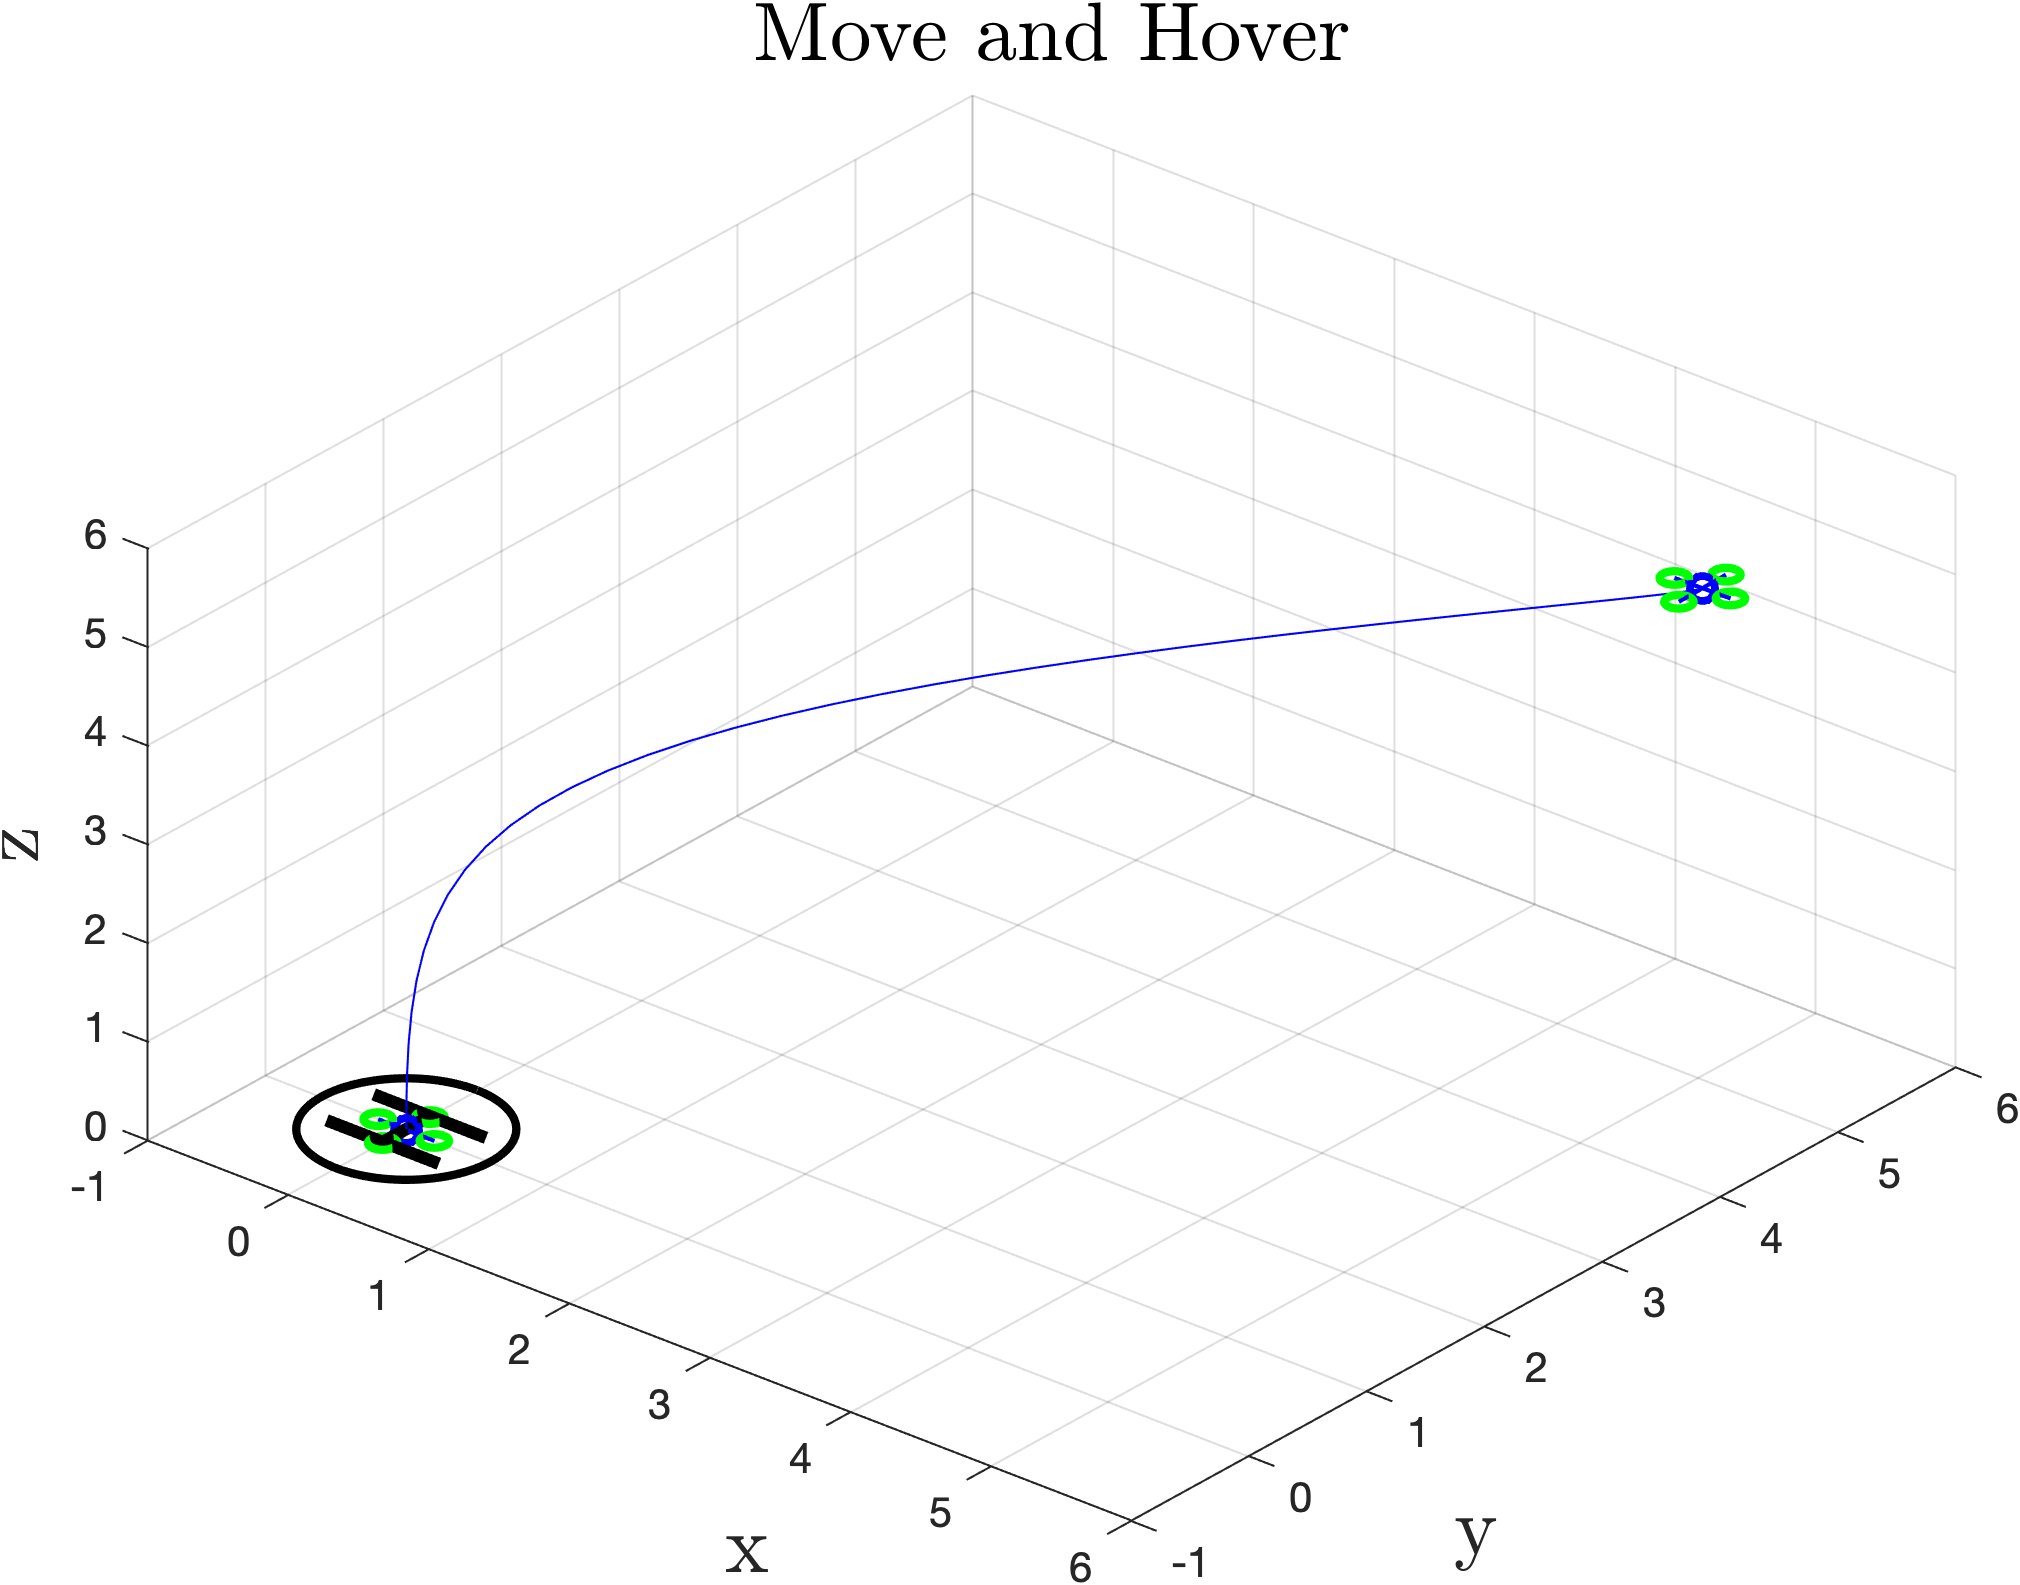
\includegraphics[width = 1\textwidth]{images/MoveAndHover.png}
     \label{fig:MandH}
     \caption{Quadrotor Move and Hover}
\end{subfigure}
\begin{subfigure}[b]{0.31\textwidth}
    \centering
    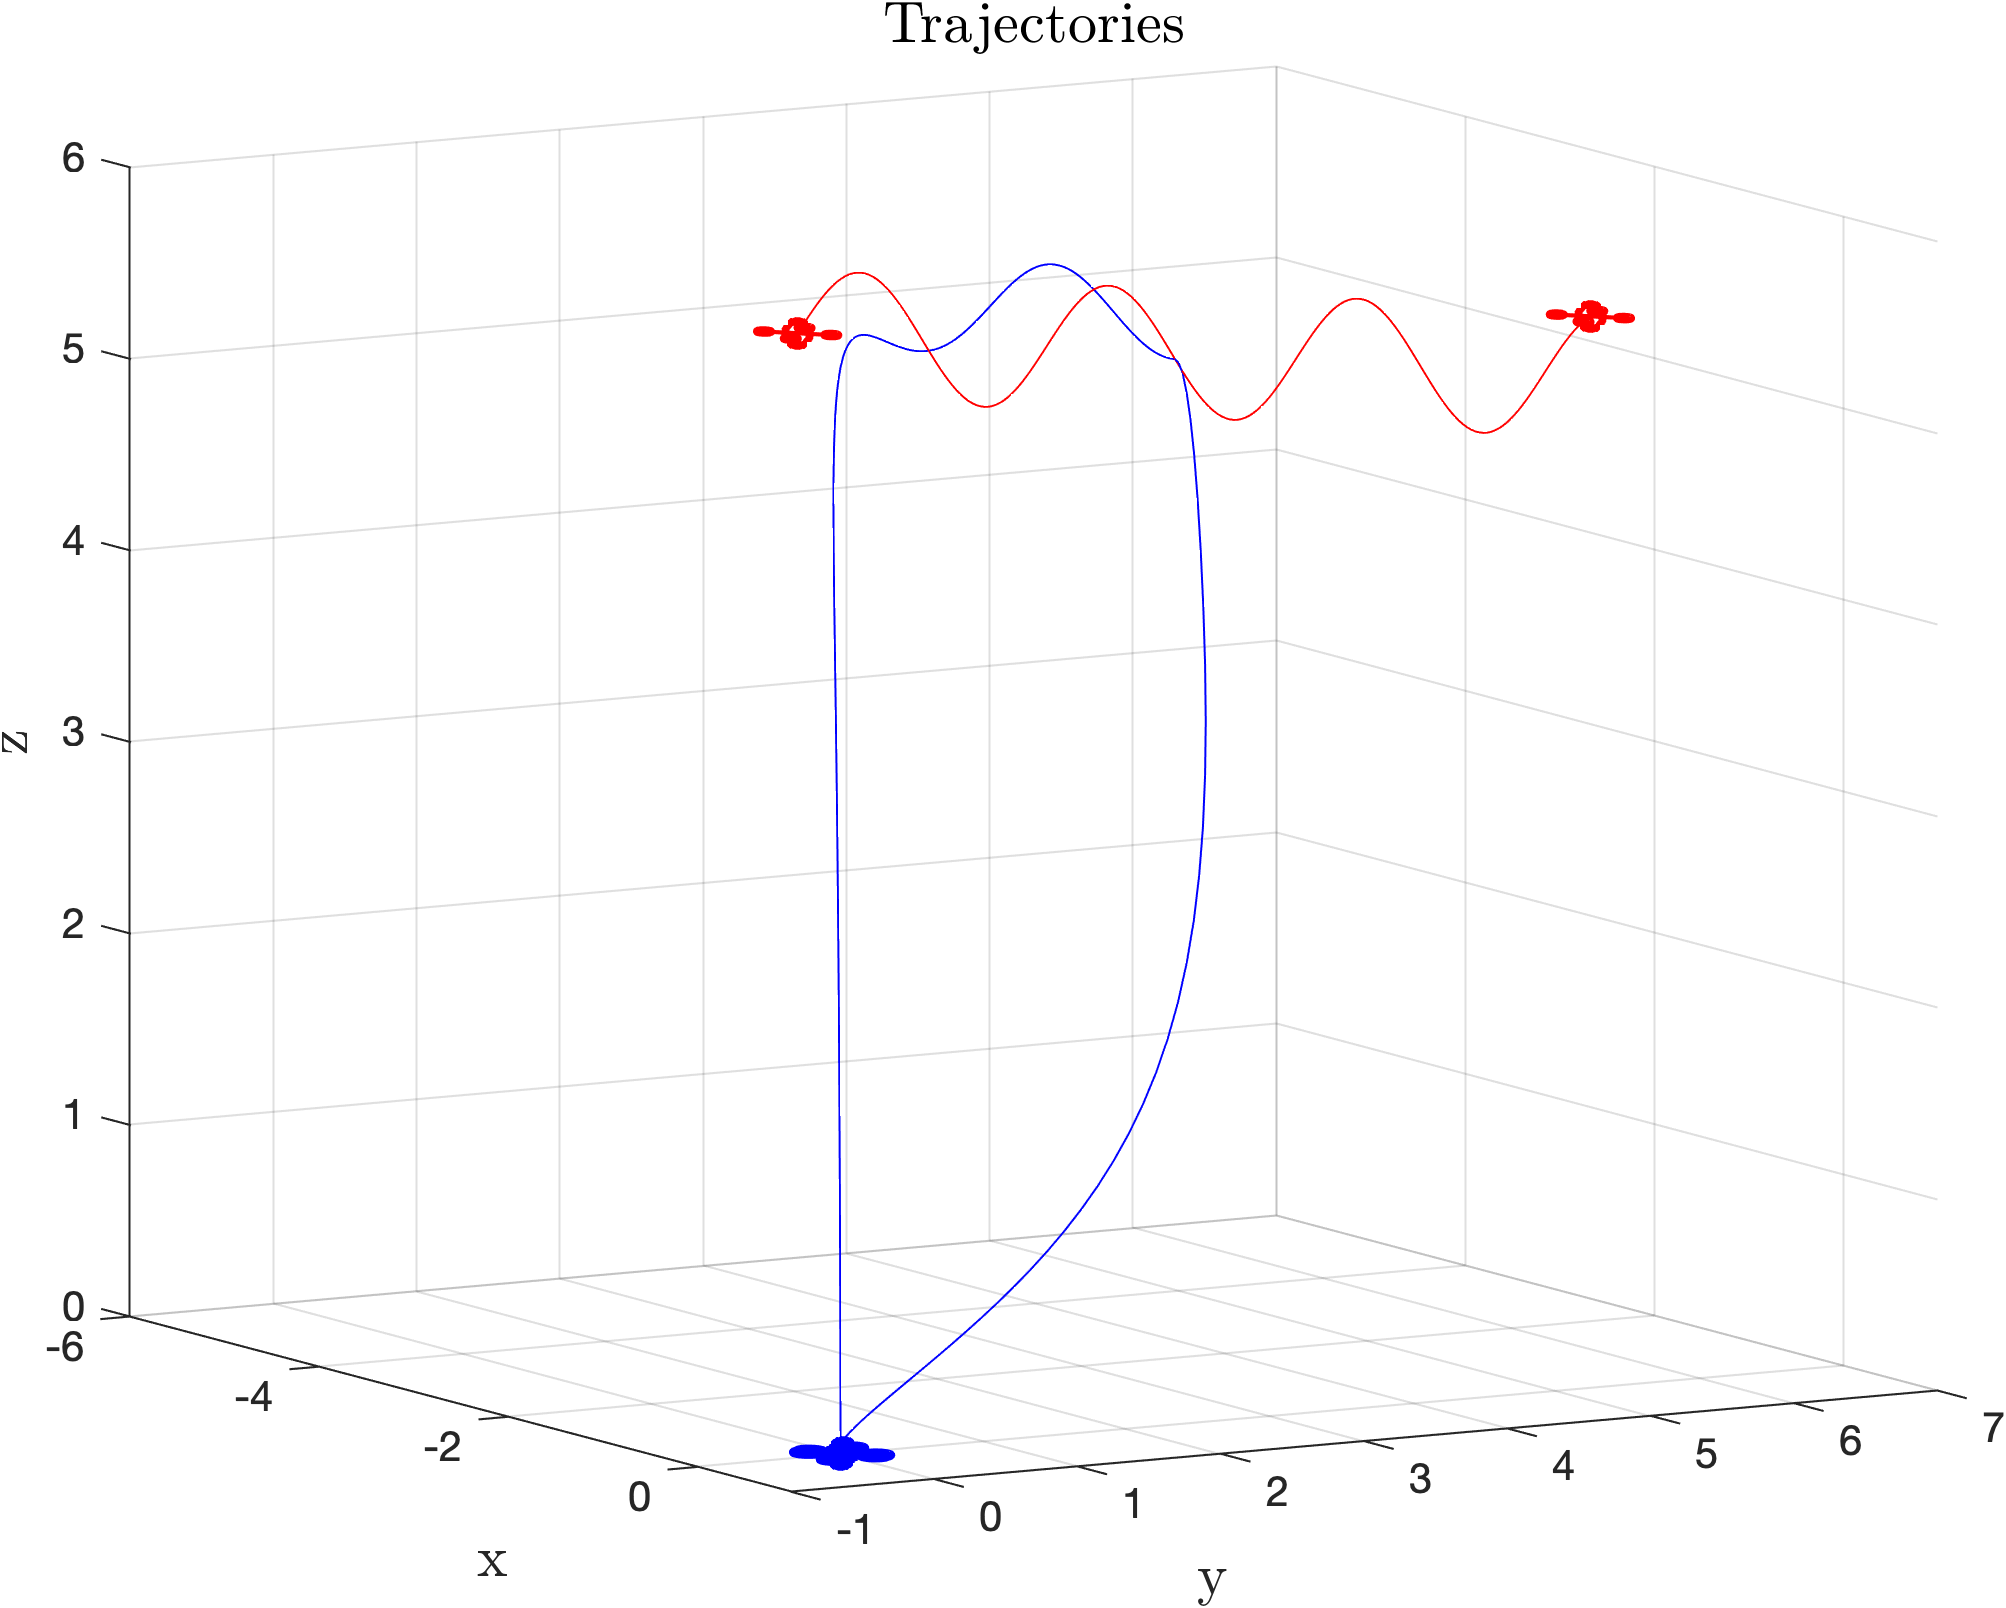
\includegraphics[width = 1\textwidth]{images/ReturnToBase.png}
     \label{fig:Return}
     \caption{Return to Base}
 \end{subfigure}
\begin{subfigure}[b]{0.31\textwidth}
    \centering
    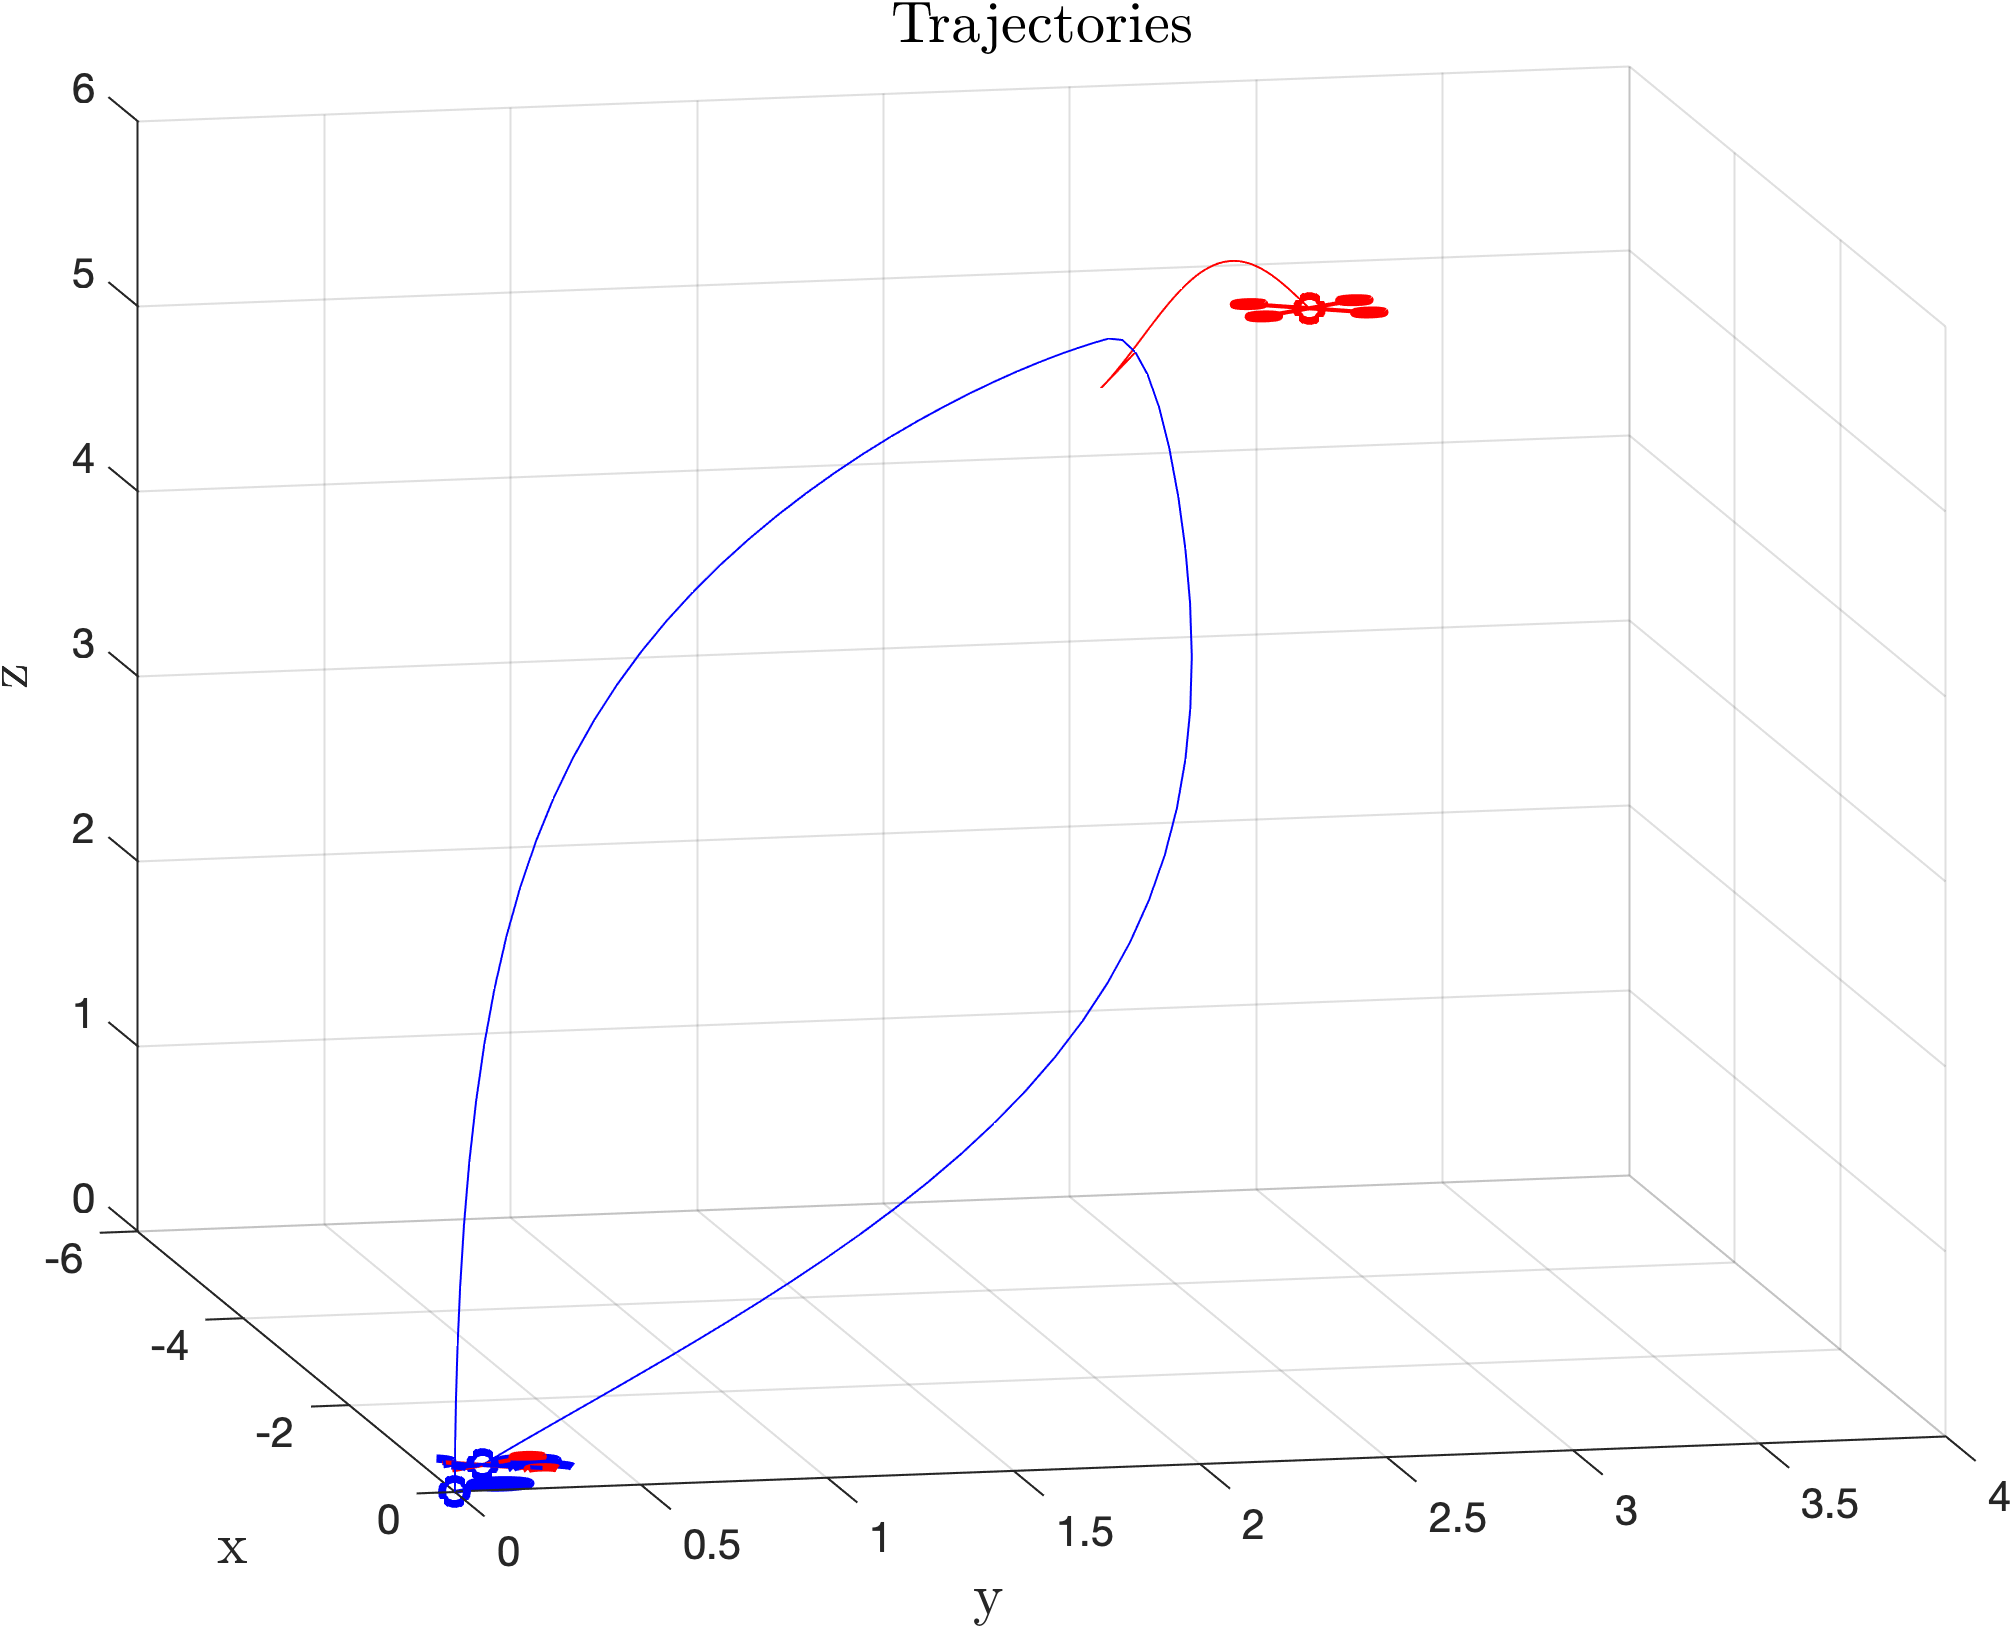
\includegraphics[width = 1\textwidth]{images/Intercept.png}
     \label{fig:Capture}
     \caption{Quadrotor Capture}
 \end{subfigure}
   \caption{Quadrotor Performance Tests}
\end{figure}

\bigskip
\section*{Quadrotor Return to Base with a Disturbance Force}
For the disturbance forces and torques after capture,  in the control of the ODE function we trigger an change in $n$ and $r$ and re-evaluate K before adding the mass of the target drone to recalculate the control, $u$, term for the ODE.  Again we use the simplification of a time dependent function for the $n$ term $n=[\sin(t)/10; \cos(t)/10; \sin(t)/10]$ to simulate the target trying to escape.  Where the terms of $n$ are in the order of 1/10 $\sin$ and $\cos$ the interceptor handles the torque well.  On the order of 1/5, initial movements after capture are handled well, but as the interceptor slows to land it has more trouble maintaining control.  At a full 2N torque(represented as 1/1) the system becomes unstable. Between 1/5 and 1/1, the interceptor combination returns close to base but crashes before reaching coordianates (0,0) in the (x,y) even with greater penalties in the $z$ section of the Q matrix.\\
  
\textbf{(End current edits)}
\section*{Results}
\section*{Discussion}

\label{References}
\bibliographystyle{abbrv}
\begin{thebibliography}{10}
\bibitem{JKim}
Jinho Kim, S. Andrew Gadsden, Stephen A . Wilkerson.
"A Comprehensive Survey of Control Strategies for Autonomus Quadrotors".
arXiv:2005.09858v1.
20 May 2020.
\bibitem{AHM}
Faraz Ahmad, Pushpendra Kumar, Anamika Bhandari, Pravin P. Patil.
Simulation of the Quadrotor Dynamics with LQR based Control.
Materials Today: Proceedings,Volume 24, Part 2, 2020, Pages 326-332,
ISSN 2214-7853.
https://doi.org/10.1016/j.matpr.2020.04.282.
\bibitem{OKY}
Okyere, E., Bousbaine, A., Poyi, G. T., Joseph, A. K., and Andrade.,
J. M. (2018) ‘LQR controller design for quad-rotor helicopters’,
The 9th International Conference on Power Electronics, Machines
and Drives. The Arena and Convention Centre, Liverpool, 17-19
April. London: The Institute of Engineering and Technology, pp.1-7
\bibitem{SUI}
Suicez, Emre Can.  Trajectory Tracking of a Quadrotor Unmanned Aerial Vehicle (UAV) via Attitude and Position Control.  Thesis for MS in Aerospace Engineering.  Middle East Technical University. July 2014. Pages 57-58.
\bibitem{Mart}
Luís Martins, Carlos Cardeira, Paulo Oliveira,
Linear Quadratic Regulator for Trajectory Tracking of a Quadrotor,
IFAC-PapersOnLine,
Volume 52, Issue 12, 2019,Pages 176-181,ISSN 2405-8963,
https://doi.org/10.1016/j.ifacol.2019.11.195.
\bibitem{kon}
Kong, Chuin-Wei.  2021, May 25. Title of video Quadcopter Simulation and Control-LQR Controller. YouTube. https://www.youtube.com/watch?v=oixM0DKNMGM
\bibitem{AHM}
Abbot, Jake. 2012, April 7. LQR Method. YouTube. https://www.youtube.com/watch?v=St5L-ekOKGA
\bibitem{MLT}
Matlab Tech Talks. 2019, February 5. Optimal Control LQR. YouTube. https://www.youtube.com/watch?v=


\end{thebibliography}

\end{multicols}

\end{document}